\subsection{SEMI-CONTINUOUS FUNCTIONS}

Let \(f\) be a real-valued function defined on a topological space \(\mathbf{X}\) . For \(f\) to be continuous at a point \(a \in \mathbf{X}\) it is necessary and sufficient that: (i) given any real number \(h < f(a)\) , there exists a neighbourhood \(\mathbf{V}\) of \(a\) such that at each point \(x \in \mathbf{V}\) we have \(h < f(x)\) ; (ii) given any real number \(k > f(a)\) , there exists a neighbourhood \(\mathbf{W}\) of \(a\) such that at each point \(x \in \mathbf{W}\) we have \(k > f(x)\) .

Functions which satisfy only one of these conditions play an important part in analysis. To be precise, we make the following definition:

DEFINITION 1. A real-valued function \(f\) , defined on a topological space \(\mathbf{X}\) , is said to be lower semi-continuous (resp. upper semi-continuous) at a point \(a \in \mathbf{X}\) , if for each \(h < f(a)\) {[}resp. each \(k > f(a)\) {]} there is a neighbourhood \(\mathbf{V}\) of a such that \(h < f(x)\) {[}resp. \(k > f(x)\) {]} for each \(x \in \mathbf{V}\) .

A real-valued function is said to be lower semi-continuous (resp. upper semi-continuous) on X if it is lower semi-continuous (resp. upper semi-continuous) at every point of X.

A real-valued function \(f\) is therefore continuous at a point \(a\) if and only if it is both upper and lower semi-continuous at \(a\) .

If \(f\) is lower semi-continuous at a point, then \(-f\) is upper semi-continuous at this point, and conversely; hence we may restrict ourselves in what follows, to considering properties of lower semi-continuous functions.

It is clear that a function which is lower semi-continuous on X is also lower semi-continuous on every subspace of X.

Examples. 1) If \(f\) has a relative minimum at a point \(a\) , that is to say if there is a neighbourhood \(V\) of \(a\) such that, for each \(x \in V\) , we have \(f(a) \leqslant f(x)\) , then \(f\) is lower semi-continuous at \(a\) . In particular, if \(f(a) = -\infty\) , \(f\) is lower semi-continuous at \(a\) .

\begin{enumerate}
\def\labelenumi{\arabic{enumi})}
\setcounter{enumi}{1}
\tightlist
\item
  Define a real-valued function \(f\) on \(\mathbf{R}\) by putting \(f(x) = 0\) if \(x\) is irrational, and \(f(x) = 1 / q\) if \(x\) is rational and equal to the irreducible fraction \(p / q\) ( \(q > 0\) ). For each integer \(n > 0\) , the set of rational numbers \(p / q\) such that \(q < n\) is closed, and its points are isolated; hence for every irrational \(x\) there is a neighbourhood \(V\) of \(x\) such that \(f(y) \leqslant 1 / n\) for all \(y \in V\) , which shows that \(f\) is continuous at \(x\) ; and on the other hand, \(f\) has a relative maximum at every rational point \(x\) . Hence \(f\) is upper semi-continuous on \(\mathbf{R}\) .
\end{enumerate}

The condition for \(f\) to be lower semi-continuous at \(a\) may be expressed by saying that, for each \(h < f(a)\) , the set \(f^{-1}(]h, +\infty])\) must be a neighbourhood of \(a\) .

It is enough that this condition should be satisfied for an increasing sequence \((h_{n})\) of real numbers \(<f(a)\) which tend to \(f(a)\) .

Endow \(\overline{\mathbf{R}}\) with the topology in which the open sets are \(\varnothing\) and all open intervals of \(\overline{\mathbf{R}}\) unbounded on the right (that is, all intervals \(]a, +\infty[\) for finite \(a\) , and the interval \([- \infty, +\infty] = ] \leftarrow, \rightarrow[\) . Then the real-valued function \(f\) is lower semi-continuous at \(a\) if and only if it is continuous at \(a\) when considered as a mapping into \(\overline{\mathbf{R}}\) endowed with this topology.

PROPOSITION 1. A real-valued function \(f\) on a topological space \(\mathbf{X}\) is lower semi-continuous if and only if, for each finite real number \(k\) , \(f^{-1}([k, +\infty])\) {[}the set of all \(x \in \mathbf{X}\) such that \(f(x) > k]\) is an open set in \(\mathbf{X}\) {[}or, equivalently, \(f^{-1}([- \infty, k])\) is a closed set in \(\mathbf{X}]\) .

For this condition shows that \(f^{-1}([k, +\infty])\) is a neighbourhood of each of its points.

For \(f\) to be lower semi-continuous on \(\mathbf{X}\) it is sufficient that \(f^{-1}([k, +\infty])\) is open in \(\mathbf{X}\) for all real numbers \(k\) belonging to a dense subset of \(\mathbf{R}\) .

COROLLARY. A subset A of a topological space X is open (resp. closed) in X if and only if its characteristic function (*) \(\varphi_{A}\) is lower (resp. upper) semicontinuous on X.

For \(f_{\mathbf{A}}^{-1}([k, +\infty])\) is empty for \(k \geqslant 1\) , is equal to \(\mathbf{A}\) for \(0 \leqslant k < 1\) and is equal to \(\mathbf{X}\) for \(k < 0\) .

THEOREM 3. Let \(f\) be a lower semi-continuous function on a non-empty quasi-compact space \(\mathbf{X}\) . Then there is at least one point \(a \in \mathbf{E}\) such that \(f(a) = \inf_{x \in \mathbf{X}} f(x)\) (in other words, \(f\) attains its greatest lower bound in \(\mathbf{X}\) ).

For each \(k \in f(\mathbf{X})\) , consider the set \(\mathbf{A}_k = f^{-1}([-\infty, k])\) . These sets are non-empty and form a filter base on \(\mathbf{X}\) ; since they are closed by Proposition 1, they have at least one common point \(a\) {[}axiom (C'') for quasi-compact spaces{]}. For each \(x \in \mathbf{X}\) we have therefore \(f(a) \leqslant f(x)\) , and the theorem follows.

COROLLARY. Let \(f\) be a lower semi-continuous function on a non-empty quasicompact space \(X\) . If \(f(x) > -\infty\) for all \(x \in X\) , then \(f\) is bounded below in \(X\) .

Note that this theorem and the corresponding theorem for upper semicontinuous functions include Weierstrass's theorem as a particular case (no. 1, Theorem 1).

PROPOSITION 2. Let \(f\) and \(g\) be two real-valued functions, lower semi-continuous at a point \(a \in \mathbf{X}\) . Then the functions \(\inf(f, g)\) and \(\sup(f, g)\) are lower semi-continuous at \(a\) ; so is \(f + g\) whenever it is defined, and so is \(fg\) if \(f\) and \(g\) are \(\geqslant 0\) and the product \(fg\) is defined.

We give the proof for \(f + g\) ; the argument is analogous in the other cases. The result is clear if either \(f(a)\) or \(g(a)\) is equal to \(-\infty\) ; if not, then \(f(a) + g(a) > -\infty\) . Every finite number \(h < f(a) + g(a)\) can be written as \(h = r + s\) , where \(r < f(a)\) and \(s < g(a)\) are finite {[}it is enough to take \(s\) so that \(h - f(a) < s < g(a)\) {]}; by hypothesis, there is a neighbourhood \(V\) of \(a\) such that, for each \(x \in V\) , we have \(r < f(x)\) , and a neighbourhood \(W\) such that for each \(x \in W\) we have \(s < g(x)\) ; therefore \(h = r + s < f(x) + g(x)\) for all points \(x\) of the neighbourhood \(V \cap W\) .

In the same way we see that, if \(f\) is lower semi-continuous at a point \(a\) , and if \(f \geqslant 0\) , then \(1 / f\) is upper semi-continuous at \(a\) .

THEOREM 4. The upper envelope of a family \((f_{t})\) of functions which are lower semi-continuous at a point \(a \in \mathbf{X}\) is lower semi-continuous at \(a\) .

  Let \(g\) be the upper envelope. For each \(h < g(a)\) there is an index \(t\) such that \(h < f_{t}(a) \leqslant g(a)\) , and a neighbourhood \(V\) of \(a\) such that \(h < f_{t}(x)\) for all \(x \in V\) ; hence a fortiori \(h < g(x)\) for all \(x \in V\) .

\pandocbounded{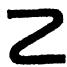
\includegraphics[keepaspectratio]{images/part003_0bad14cb.jpg}}

It follows from Proposition 2 that the lower envelope of a finite number of lower semi-continuous functions is again lower semi-continuous; but this is not in general true for the lower envelope of an infinite family of lower semi-continuous functions. For example, if r is any rational number, let \(f_{r}\) denote the function which is equal to 0 at r and equal to 1 for all real numbers \(x \neq r\) ; the lower envelope of the \(f_{r}\) is the function g which is equal to 0 for every rational number and 1 for every irrational number (``Dirichlet's function''), and this function is not lower semi-continuous at irrational points.

COROLLARY. The upper envelope of a family of continuous real-valued functions on a space X is lower semi-continuous on X.

In Chapter IX, § 1, no. 6, Proposition 5, we shall show that the converse of this proposition is true if X is uniformizable (and only in this case): every lower semi-continuous function on a uniformizable space is the upper envelope of a family of continuous functions.

PROPOSITION 3. A real-valued function \(f\) , defined on a topological space \(\mathbf{X}\) , is lower semi-continuous at a point \(a \in \mathbf{X}\) if and only if \(\liminf_{x \to a} f(x) = f(a)\) {[}or, equivalently, if and only if \(\liminf_{x \to a} f(x) \geqslant f(a)\) {]}.

The condition is necessary. For, given any \(h < f(a)\) , there is a neighbourhood \(V\) of \(a\) such that \(h < f(x)\) for all \(x \in V\) ; therefore

\[
h \leqslant \inf _ {x \in \mathbf {V}} f (x) \leqslant \liminf _ {x \rightarrow a} f (x)
\]

(§ 5, no. 6, formulae (12)), and so \(f(a) \leqslant \liminf_{x \to a} f(x)\) . The condition is sufficient; for if it is satisfied, then for each \(h < f(a)\) there is a neighbourhood \(V\) of \(a\) such that \(h \leqslant \inf_{x \in V} f(x)\) , and therefore \(f\) is lower semicontinuous at \(a\) .

PROPOSITION 4. Let \(f\) be any real-valued function defined on a dense subset \(A\) of a topological space \(X\) . If, for each \(x \in X\) , we put \(g(x) = \liminf_{y \to x, y \in A} f(y)\) , then \(g\) is lower semi-continuous on \(X\) .

For, given any \(h < g(x)\) , there is an open neighbourhood \(\mathbf{V}\) of \(x\) such that, for all \(z \in \mathbf{V} \cap \mathbf{A}\) , we have \(h < f(z)\) ; now \(\mathbf{V}\) is a neighbourhood of each of its points \(y\) ; thus we have \(\liminf_{z \to y, z \in \mathbf{A}} f(z) = g(y) \geqslant h\) for all \(y \in \mathbf{V}\) , and the result follows.

The function g is called the lower semi-continuous regularization of f.~We define the upper semi-continuous regularization of f similarly.

We may also define \(g\) as the greatest of the lower semi-continuous functions \(\varphi\) on \(\mathbf{X}\) which are such that \(\varphi(x) \leqslant f(x)\) for all \(x \in \mathbf{A}\) . If \(f\) is lower semi-continuous on \(\mathbf{A}\) , then \(g\) is an extension of \(f\) to \(\mathbf{X}\) , by Proposition 3.

